\chapter{First increment}
\label{chap:First Increment}
Test om: Bounce, predefined area
Skal komme væk fra accelerotmeter og gyroscope. 

\section{Requirements}
\label{sec:i1Requirements}
The requirements which will be considered in this increment is mark with a blue colour.

\begin{itemize}
\item The trash bin should catch the trash if the user throws it towards the trash bin and within a predefined area
\begin{itemize}
\item \textcolor{blue}{The robots predefined area should be calculated from the hardware limitations of the motors’ speed}
\end{itemize}
\item The robot should know where it is positioned
\begin{itemize}
\item \textcolor{blue}{The robot should have a starting position, from where it should be able to calculate it's current position}
\end{itemize}
\item The robot should be able to detect and track the thrown trash
\begin{itemize}
\item \textcolor{blue}{The thrown trash should be detected and tracked by a Microsoft Kinect}
\item The Kinect should send the coordinates of the impact point of the trash to the robot
\end{itemize}
\item The robot should know where the the thrown trash will land
\begin{itemize}
\item \textcolor{blue}{Trajectory prediction should be used to calculate impact point of the thrown trash}
%\item \textcolor{red}{The trajectory prediction should include a bounce prediction}
%\item \textcolor{red}{The bounce-shot should be thrown from a designated side of the camera}
%\item \textcolor{red}{The bounce-shot should bounce into the predefined area where the robot should catch the trash within }
\end{itemize}
\item The robot should be able to move the trash bin, such that the thrown trash lands inside the bin
\begin{itemize}
\item \textcolor{blue}{The robot should be able to turn, drive forward and drive backwards}
\item Multiple trash thrown should not be considered
\end{itemize}
\end{itemize}

These requirements are rudimentary, and the very essence of the project lies within the fulfilment of these requirements. In this increment the fundamentals of the robot’s movement should be implemented, the predefined area should be calculated, a starting point for this area should be determined and the Microsoft Kinect should be able to detect and track an object with the use of trajectory prediction.

\section{System design}
\label{sec:i1System Design}

\subsection{Throwing}
\label{sec:i1Throwing}
Test have been made to ensure that the robot is provided the most time for the calculations and catching the trash. In order to do so, multiple test were conducted, and the results were acquired from a distance of 3 meter, the time it took for the trash (in this case, a table tennis ball) was in average 1.1 second. Multiple tests from a distance of 5 meter were also conducted and that provided an average of 1.25 second. 

With the results from the throwing tests, the group could conclude that a normal throw wouldn't serve the robot enough time to catch the ball, else the predefined area for the robot had to be very small, due to the limitations of the motors. As mentioned in the \ref{sec:LEGO NXT Servo motor} section, the group calculated the robot's speed to be ~87 RPM, which simply isn't enough to catch trash from a 3 or 5 meter distance. The robot would be able to catch trash within 280mm of itself, given the 1.1 second run time, for the 3 meter throw, and therefore nowhere near sufficient enough. 

The group decided after several tests to let the trash (still a table tennis ball) be bounced on the floor before it had to be catched, which would give the robot extra time to get to the collision point of the ball. This provided in nearly the amount the double amount of time for the throw to be catched, providing an average of 2s from a 3 meter throw and 2.15s from a 5m throw.

\subsection{Predefined area}
\label{sec:i1Predefined area}
The robots predefined area, is a field where the robot should catch the ball within. As mentioned in  section \ref{sec:i1Throwing}, the bouncing throw would have a travel time of 2 - 2.15 seconds, before landing in the predefined area. The predefined area was calculated using the robot itself. The robot was placed marking its starting point, which will be its starting point every time. It was set to turn a specific number of degrees and moving forward, after two seconds the robot would stop. The place the robot stops is marked aswell, which lead to the predefined area seen in figure \label{figure:Predefined area}.

\begin{figure}[h]
\centering
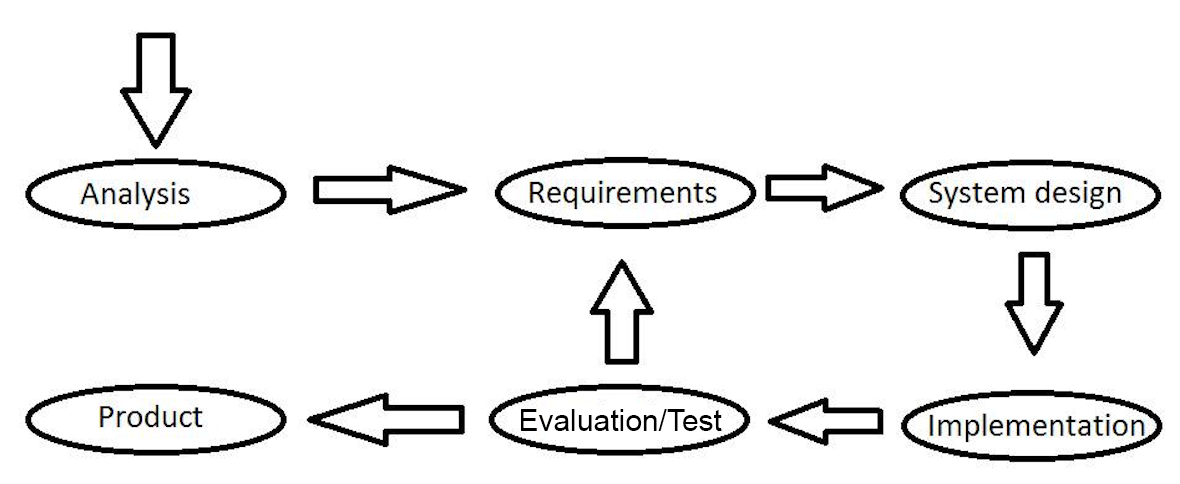
\includegraphics[scale=0.35]{billeder/process-model}
\caption{Process model used for the project}
\label{pm}
\end{figure}

\section{Implementation}
\label{sec:i1Implementation}

\section{Evaluation}
\label{sec:i1Evaluation}
